\documentclass[conference]{IEEEtran}
\IEEEoverridecommandlockouts
\usepackage[utf8]{inputenc}
\usepackage[T1]{fontenc}
\usepackage[brazil]{babel}
\usepackage{cite}
\usepackage{amsmath,amssymb,amsfonts}
\usepackage{algorithmic}
\usepackage{graphicx}
\usepackage{textcomp}
\usepackage{xcolor}
\usepackage{booktabs}
\usepackage{url}
\def\BibTeX{{\rm B\kern-.05em{\sc i\kern-.025em b}\kern-.08em
    T\kern-.1667em\lower.7ex\hbox{E}\kern-.125emX}}
\graphicspath{{figures/}}
% Rótulos em português no estilo IEEE
\addto\captionsbrazil{\renewcommand{\IEEEkeywordsname}{Palavras-chave}}
\renewcommand{\IEEEkeywordsname}{Palavras-chave}

\begin{document}

\title{Quinze Jogos Não São uma Temporada: Previsão da Classificação da NBA e das Chances de Playoff com Regressão Regularizada e Simulação de Monte Carlo}

\author{\IEEEauthorblockN{[Nome do Autor 1]}
\IEEEauthorblockA{\textit{Universidade Federal do ABC (UFABC)}\\
São Bernardo do Campo, Brasil \\
[e-mail ou RA]}
\and
\IEEEauthorblockN{[Nome do Autor 2]}
\IEEEauthorblockA{\textit{Universidade Federal do ABC (UFABC)}\\
São Bernardo do Campo, Brasil \\
[e-mail ou RA]}
}

\maketitle

\begin{abstract}
Depois de cerca de quinze jogos de uma temporada regular da NBA, a classificação é dominada por ruído, mas torcedores, imprensa e times já tiram conclusões dela. Investigamos quão bem é possível prever, nesse ponto da temporada 2026--27, o aproveitamento final de cada time e sua probabilidade de terminar entre os seis primeiros, na zona de play-in ou fora da pós-temporada de sua conferência. Com dezesseis temporadas de dados jogo a jogo coletados pela biblioteca nba\_api, construímos seis features a partir dos quinze primeiros jogos de cada time e comparamos dois baselines ingênuos com regressão linear, Ridge, Lasso e random forest, sob validação leave-one-season-out e holdout temporal. Todos os modelos treinados reduzem o erro absoluto médio de 7,6 para cerca de 5,6 vitórias em escala de 82 jogos; escolhemos o Ridge, cuja penalidade estabiliza features quase colineares baseadas em pontos sem perda de precisão. Alimentando um modelo logístico de jogo com as previsões do Ridge e simulando 10.000 vezes o restante do calendário, obtemos probabilidades bem calibradas em um backtest fora da amostra, com cobertura de 81\% para intervalos nominais de 80\%.
\end{abstract}

\begin{IEEEkeywords}
análise esportiva, regressão Ridge, regressão à média, validação cruzada, simulação de Monte Carlo, basquete
\end{IEEEkeywords}

%=====================================================================
\section{Introdução}
Todo mês de novembro, alguns times da NBA começam muito acima ou muito abaixo do esperado. Um começo 14--3 é sinal de candidato ao título ou uma boa fase que vai passar? A pergunta vai além da torcida: dirigentes decidem se compram ou vendem jogadores antes do prazo de trocas, e as narrativas da imprensa se formam cedo. Estatisticamente, é um caso clássico de \emph{regressão à média}: o aproveitamento no início da temporada é uma medida ruidosa da força do time, e valores extremos tendem a voltar para a média da liga~\cite{efron1975,efron1977}.

Estudamos a seguinte pergunta: \emph{com cerca de 15 jogos disputados na temporada 2026--27 da NBA, qual será o aproveitamento final de cada time e qual a probabilidade de cada um terminar entre os seis primeiros (vaga direta nos playoffs), no torneio play-in (7º--10º) ou fora, em sua conferência?}

A abordagem tem duas etapas. Primeiro, um modelo de regressão supervisionado relaciona a informação disponível após $N=15$ jogos ao aproveitamento final. Tratamos isso como um problema de encolhimento (\emph{shrinkage}), para o qual modelos lineares regularizados como o Ridge~\cite{hoerl1970} são naturais, e os comparamos com baselines, Lasso~\cite{tibshirani1996} e random forests~\cite{breiman2001}. Depois, as forças previstas alimentam um modelo logístico de jogo e uma simulação de Monte Carlo~\cite{metropolis1949} do calendário restante, transformando previsões pontuais em probabilidades de posição na conferência. As duas etapas são validadas fora da amostra, incluindo um backtest da simulação completa em dezesseis temporadas passadas.

%=====================================================================
\section{Dados}
\subsection{Fonte e coleta}
Usamos o endpoint \texttt{LeagueGameLog} do cliente Python de código aberto \texttt{nba\_api}~\cite{nbaapi}, que acessa o serviço oficial \url{stats.nba.com}, para coletar o box score por time de todos os jogos de temporada regular de 2010--11 a 2025--26 (16 temporadas completas) e da temporada 2026--27 até 22 de novembro de 2026. Cada linha time-jogo traz data, adversário, mando de quadra, resultado, pontos, arremessos de quadra e lances livres tentados, rebotes ofensivos e erros de ataque. As requisições foram espaçadas em um segundo, repetidas com espera exponencial em caso de falha e armazenadas em cache, um CSV por temporada. O calendário restante de 2026--27 (952 jogos) veio do endpoint \texttt{ScheduleLeagueV2}. Siglas de franquias que mudaram no período (NJN$\to$BKN, NOH$\to$NOP) foram normalizadas, e cada time foi associado à sua conferência. A amostra histórica tem 38.238 linhas time-jogo (19.119 jogos).

\subsection{Unidade de análise e alvo}
Seja $N$ o menor número de jogos disputados por um time em 2026--27 no momento da coleta; aqui $N=15$ (os times tinham de 15 a 18 jogos). Cada observação é um time-temporada (480 históricos e 30 atuais). O alvo é o \emph{aproveitamento final} $y$, e não o número de vitórias, porque três temporadas foram encurtadas (66 jogos por time em 2011--12, de 64 a 75 em 2019--20 e 72 em 2020--21). Os erros são reportados em vitórias na escala de 82 jogos, isto é, $82\,|y-\hat y|$.

\subsection{Features}
Todas as features usam apenas os $N$ primeiros jogos de cada time; nenhuma informação posterior ao $N$-ésimo jogo do time entra em qualquer feature:
\begin{itemize}
\item \textbf{Aproveitamento} após $N$ jogos.
\item \textbf{Saldo de pontos por jogo}, $(\mathrm{PF}-\mathrm{PA})/N$.
\item \textbf{Net rating}, $100(\mathrm{PF}-\mathrm{PA})/\mathrm{Posses}$, com posses estimadas por~\cite{kubatko2007}
\begin{equation}
\mathrm{Posses} \approx \mathrm{FGA} + 0{,}44\,\mathrm{FTA} - \mathrm{OREB} + \mathrm{TOV},
\label{eq:poss}
\end{equation}
na média entre os dois times.
\item \textbf{Pythagorean expectation}~\cite{kubatko2007},
\begin{equation}
\mathrm{Pyth} = \frac{\mathrm{PF}^{14}}{\mathrm{PF}^{14}+\mathrm{PA}^{14}} = \frac{1}{1+(\mathrm{PA}/\mathrm{PF})^{14}},
\label{eq:pyth}
\end{equation}
em que a forma da direita evita estouro numérico.
\item \textbf{Força de tabela}: aproveitamento médio dos adversários enfrentados, calculado só com jogos disputados até a data do $N$-ésimo jogo do time e sem contar os jogos contra o próprio time.
\item \textbf{Aproveitamento da temporada anterior} (a temporada 2009--10 também foi coletada para isso).
\end{itemize}
A Fig.~\ref{fig:corr} mostra que as três features baseadas em pontos são quase perfeitamente colineares ($r>0{,}99$) e que a força de tabela após 15 jogos praticamente não se correlaciona com o resultado final.

\begin{figure}[t]
\centerline{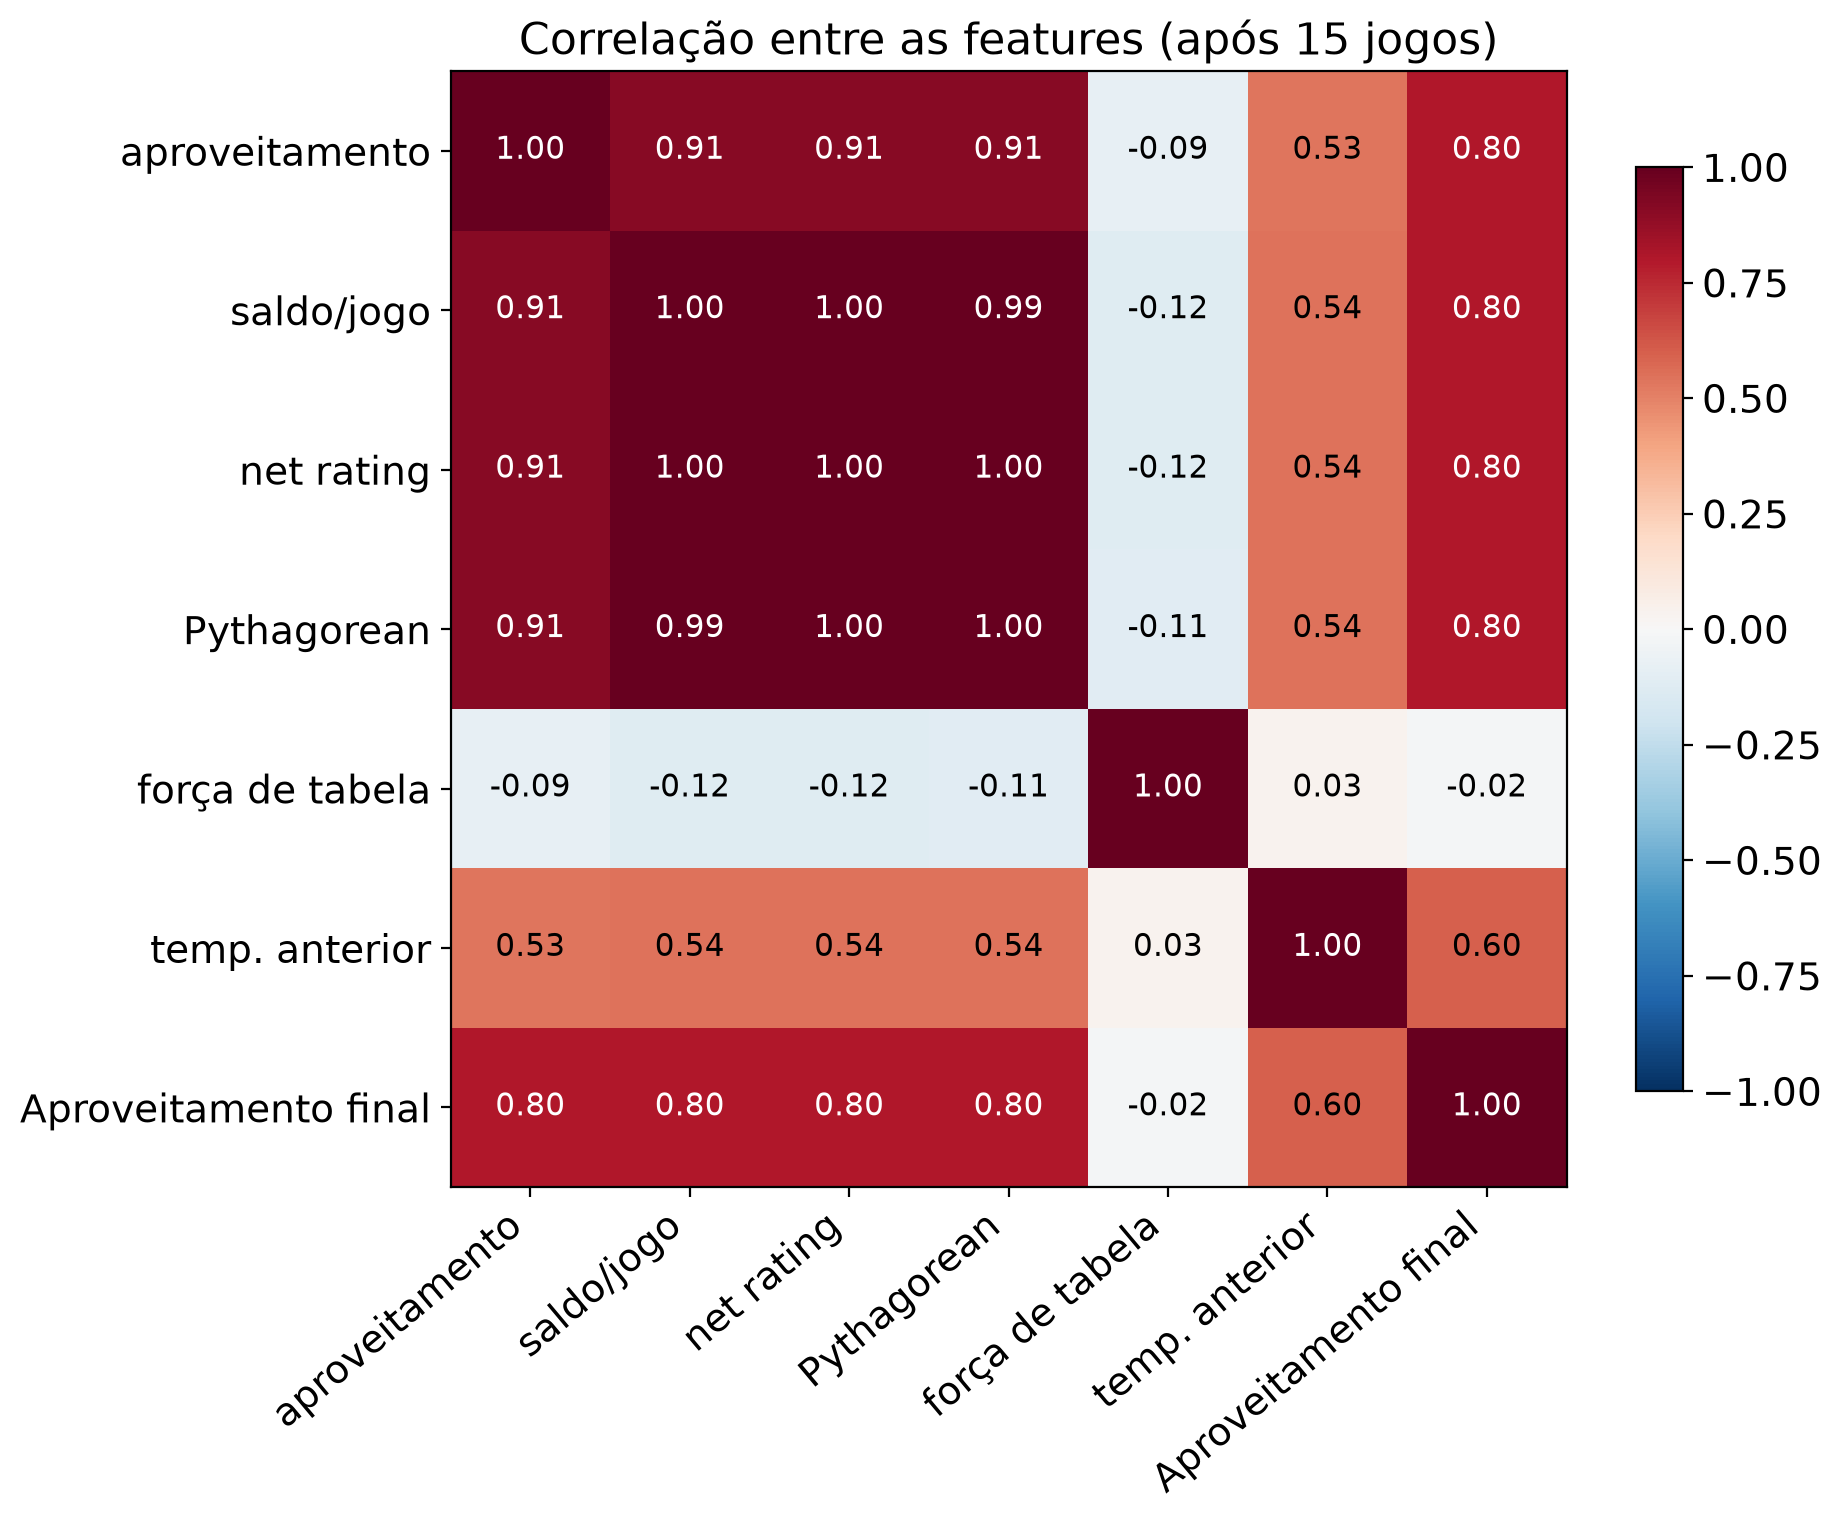
\includegraphics[width=0.92\columnwidth]{correlacao_features.png}}
\caption{Correlação de Pearson entre as features após 15 jogos e o aproveitamento final (480 times-temporada históricos).}
\label{fig:corr}
\end{figure}

%=====================================================================
\section{Método}
\subsection{Por que encolhimento}
A Fig.~\ref{fig:rtm} mostra o aproveitamento final contra o aproveitamento após 15 jogos. A inclinação de mínimos quadrados é 0,63 e a reta cruza $y=x$ perto de 0,500: cada ponto acima ou abaixo de 0,500 após 15 jogos vale só cerca de 63\% de um ponto no fim da temporada. O desvio-padrão do aproveitamento cai de 0,190 após 15 jogos para 0,151 no fim. Um bom preditor precisa, portanto, \emph{encolher} as campanhas iniciais em direção à média. É exatamente isso que modelos de regressão aprendem; a questão é como combinar vários sinais ruidosos e colineares.

\begin{figure}[t]
\centerline{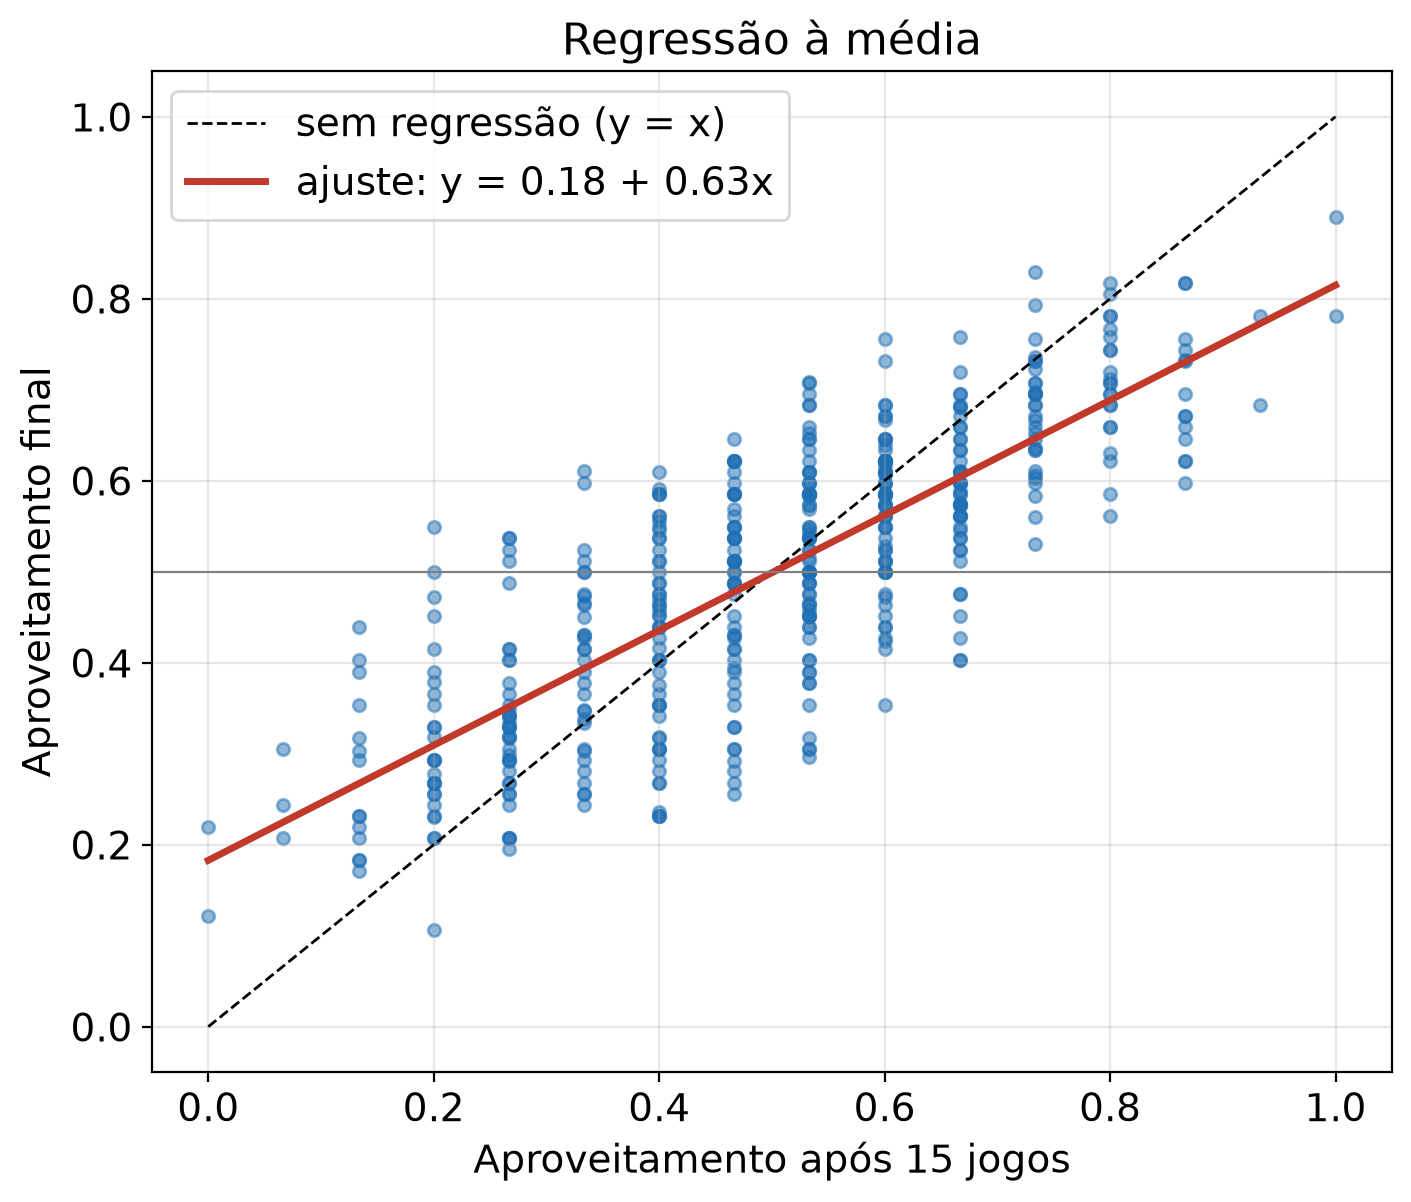
\includegraphics[width=0.85\columnwidth]{regressao_a_media.png}}
\caption{Regressão à média: aproveitamento final contra aproveitamento após 15 jogos. A inclinação ajustada (0,63) fica bem abaixo da reta identidade.}
\label{fig:rtm}
\end{figure}

\subsection{Modelos}
Comparamos dois baselines e quatro regressores treinados:
\begin{itemize}
\item \textbf{Baseline A}: mantém o aproveitamento atual ($\hat y = $ aproveitamento após $N$ jogos).
\item \textbf{Baseline B}: usa a Pythagorean expectation~\eqref{eq:pyth}.
\item \textbf{Regressão linear (OLS)} sobre as seis features.
\item \textbf{Regressão Ridge}~\cite{hoerl1970}, que minimiza
\begin{equation}
\sum_{i=1}^{n}\left(y_i-\beta_0-\mathbf{x}_i^{\top}\boldsymbol{\beta}\right)^2+\alpha\,\|\boldsymbol{\beta}\|_2^2 .
\label{eq:ridge}
\end{equation}
A penalidade $\ell_2$ encolhe os coeficientes e, em particular, distribui o peso entre preditores correlacionados em vez de dar a eles coeficientes grandes e de sinais opostos~\cite{islr2021,esl2009}.
\item \textbf{Lasso}~\cite{tibshirani1996}, com penalidade $\ell_1$, que pode zerar coeficientes.
\item \textbf{Random forest}~\cite{breiman2001} com 500 árvores, folha mínima de 10 observações e 50\% das features por divisão, como checagem não linear.
\end{itemize}
Todas as features são padronizadas dentro de um \texttt{Pipeline} do scikit-learn~\cite{sklearn}, de modo que os parâmetros de escala são aprendidos apenas nas dobras de treino.

\subsection{Protocolo de validação}
Times-temporada de uma mesma temporada compartilham condições da liga (mudanças de regra, ritmo de jogo, a ``bolha'' de 2020), então a temporada é a unidade natural de agrupamento. Usamos (i) validação cruzada \textbf{leave-one-season-out} (LOSO), com 16 dobras, e (ii) um \textbf{holdout temporal}, treinando de 2010--11 a 2022--23 e testando de 2023--24 a 2025--26. A força de regularização $\alpha$ do Ridge e do Lasso é escolhida por um \texttt{GroupKFold} \emph{interno} (5 dobras, agrupadas por temporada) dentro de cada conjunto de treino externo, ou seja, validação cruzada aninhada. Como a curva de validação interna é quase plana para $\alpha$ pequeno, aplicamos a \textbf{regra de um erro-padrão}~\cite{esl2009}: o maior $\alpha$ cujo erro fica a até um erro-padrão do mínimo.

Reportamos o MAE em vitórias (escala de 82 jogos) e a correlação de Spearman entre a classificação prevista e a real, calculada por temporada e conferência e depois promediada. Entre os modelos treinados cujo MAE LOSO fica a até um erro-padrão (entre temporadas) do melhor, escolhemos o mais regularizado (ordem de preferência: Ridge, Lasso, OLS, random forest).

\subsection{Das previsões às chances de playoff}
\paragraph{Modelo de jogo} Cada time recebe um rating $r$ igual ao seu aproveitamento final previsto. Nas temporadas históricas usamos as previsões LOSO, fora da amostra, para evitar vazamento. A probabilidade de o time $A$ vencer o time $B$ é modelada por uma regressão logística, no espírito do modelo de Bradley--Terry~\cite{bradley1952},
\begin{equation}
\mathrm{logit}\,P(A \text{ vence}) = b_{\Delta}\,(r_A - r_B) + b_{h}\,h,
\label{eq:logit}
\end{equation}
em que $h=+1$ se $A$ joga em casa e $-1$ caso contrário; o intercepto é omitido por simetria. O modelo é ajustado em todos os jogos históricos disputados após o $N$-ésimo jogo de ambos os times (30.790 linhas time-jogo).

\paragraph{Incerteza do rating} O rating também é uma estimativa. Decompomos a variância do resíduo LOSO do aproveitamento final em erro de rating e sorte jogo a jogo,
\begin{equation}
\mathrm{Var}(y-\hat y) \approx f^2\sigma^2 + \frac{\overline{y(1-y)}\,(82-N)}{82^2}, \quad f=\frac{82-N}{82},
\label{eq:sigma}
\end{equation}
e resolvemos para $\sigma$. Em cada simulação, cada rating recebe uma perturbação $\mathcal{N}(0,\sigma^2)$.

\paragraph{Monte Carlo} Simulamos os 952 jogos restantes de 2026--27 10.000 vezes e somamos os resultados à campanha atual de cada time. Jogos disputados e marcados somam 80 por time: os dois últimos dependem da fase eliminatória da NBA Cup, ainda não definida, e são simulados contra um adversário médio em quadra neutra. Os times são ordenados em cada conferência, e empates são desfeitos aleatoriamente. Para cada time reportamos as vitórias esperadas, um intervalo de 80\% (percentis 10 e 90) e as probabilidades de terminar em 1º--6º, 7º--10º e 11º--15º.

\paragraph{Backtest} Para verificar a calibração, refazemos cada temporada histórica a partir da data em que o último time completou $N$ jogos, a mesma situação de 2026--27, usando ratings LOSO e reajustando o modelo de jogo~\eqref{eq:logit} e $\sigma$ sem a temporada testada. Medimos a cobertura dos intervalos de 80\% e o Brier score de três classes~\cite{brier1950}.

%=====================================================================
\section{Resultados}
\subsection{Comparação de modelos}
A Tabela~\ref{tab:models} resume os dois esquemas de validação. Os quatro modelos treinados reduzem o erro do baseline ingênuo em cerca de duas vitórias (de 7,60 para 5,50--5,72 no LOSO) e melhoram a correlação de postos. As diferenças entre eles ficam abaixo de um erro-padrão entre temporadas (0,25 vitória). O holdout temporal conta a mesma história, então os modelos não pioram nas temporadas recentes. A Fig.~\ref{fig:pvr} compara o baseline A com o Ridge: as faixas verticais do baseline, uma para cada campanha possível após 15 jogos, são comprimidas em direção à diagonal.

\begin{table}[t]
\caption{Comparação de modelos (MAE em vitórias na escala de 82 jogos; Spearman da classificação por conferência)}
\begin{center}
\begin{tabular}{lcccc}
\toprule
 & \multicolumn{2}{c}{\textbf{LOSO (16 temporadas)}} & \multicolumn{2}{c}{\textbf{Holdout 2023--26}} \\
\textbf{Modelo} & \textbf{MAE} & \textbf{Spearman} & \textbf{MAE} & \textbf{Spearman} \\
\midrule
Regressão linear (OLS) & 5{,}50 & 0{,}785 & 5{,}22 & 0{,}867 \\
\textbf{Ridge} & 5{,}62 & 0{,}784 & 5{,}35 & 0{,}864 \\
Lasso & 5{,}68 & 0{,}788 & 5{,}45 & 0{,}877 \\
Random forest & 5{,}72 & 0{,}779 & 5{,}42 & 0{,}816 \\
Baseline: Pythagorean & 6{,}83 & 0{,}749 & 6{,}13 & 0{,}819 \\
Baseline: mantém aproveitamento & 7{,}60 & 0{,}743 & 6{,}93 & 0{,}817 \\

\bottomrule
\end{tabular}
\label{tab:models}
\end{center}
\end{table}

\begin{figure*}[t]
\centerline{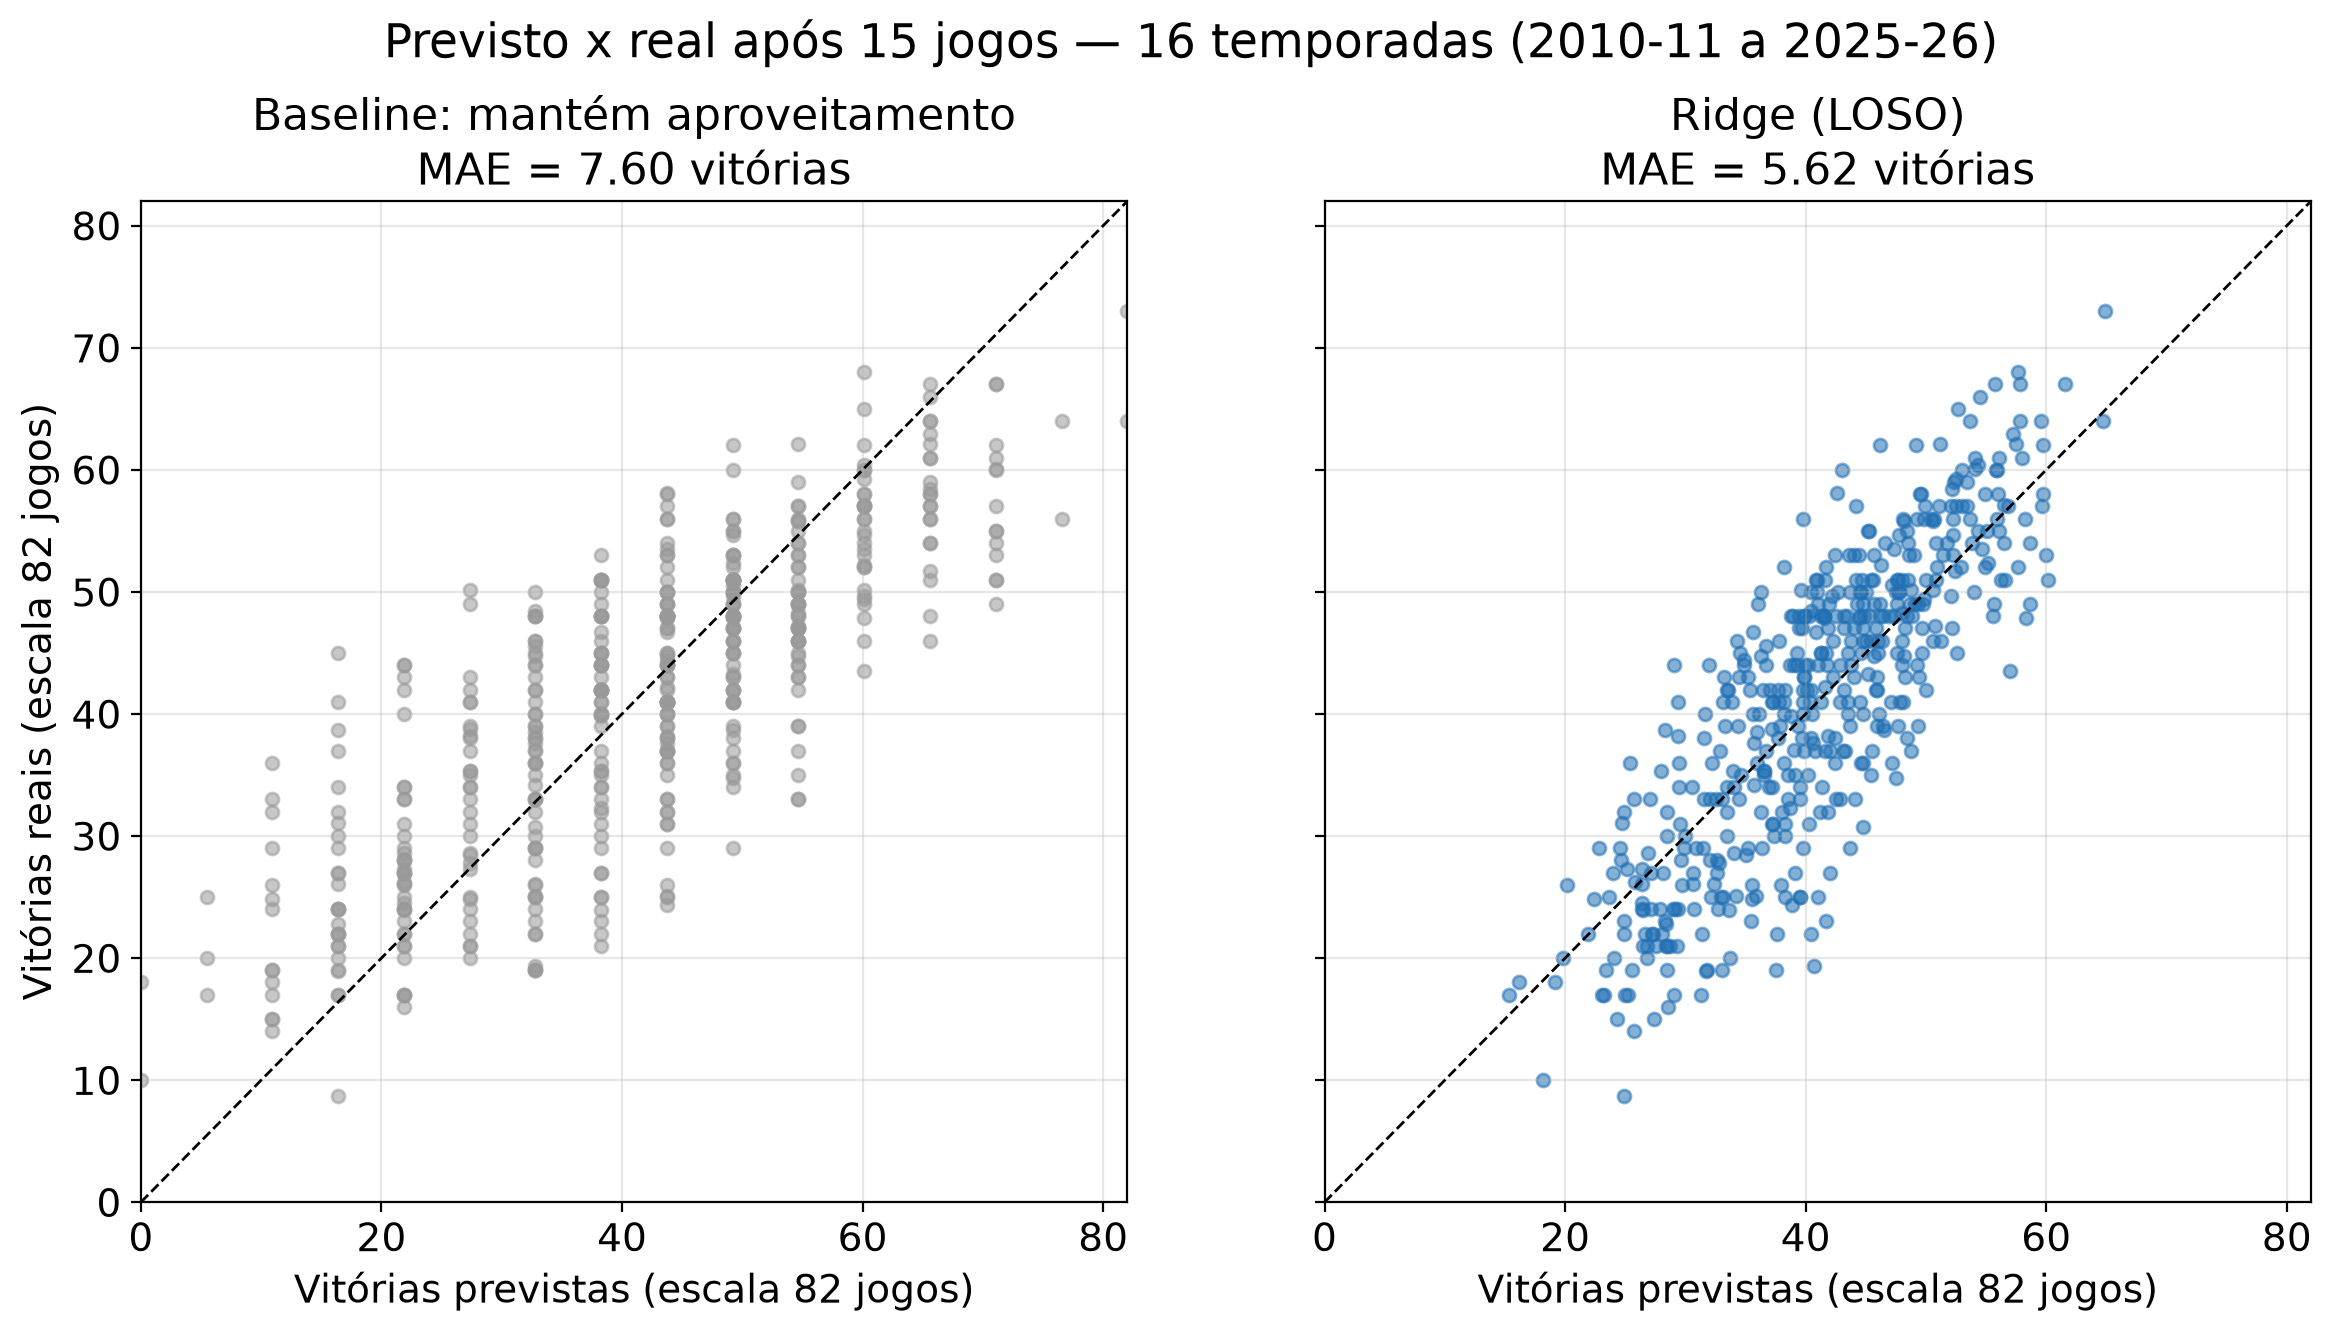
\includegraphics[width=0.85\textwidth]{previsto_vs_real.png}}
\caption{Vitórias previstas contra vitórias reais (escala de 82 jogos) nos 480 times-temporada históricos, com validação leave-one-season-out. Esquerda: baseline que mantém o aproveitamento após 15 jogos. Direita: Ridge.}
\label{fig:pvr}
\end{figure*}

\subsection{Por que Ridge}
O OLS tem o menor MAE LOSO (5,50 contra 5,62), mas a diferença está dentro do ruído, enquanto seus coeficientes não são interpretáveis (Tabela~\ref{tab:coefs}): saldo de pontos e net rating, com correlação de 0,999, recebem $+0{,}16$ e $-0{,}18$. O Ridge, com $\alpha=100$ escolhido pela regra de um erro-padrão, distribui aproximadamente o mesmo peso ($\approx0{,}023$) entre as três features baseadas em pontos, mantém o aproveitamento inicial e a temporada anterior como sinais relevantes e dá peso quase nulo à força de tabela. O intercepto é 0,500, então as previsões são encolhidas em direção à média da liga. Essa é a estabilidade esperada da regularização $\ell_2$ sob multicolinearidade~\cite{hoerl1970,islr2021}.

\begin{table}[t]
\caption{Coeficientes padronizados ajustados nos 480 times-temporada históricos}
\begin{center}
\begin{tabular}{lcc}
\toprule
\textbf{Feature} & \textbf{OLS} & \textbf{Ridge ($\alpha=100$)} \\
\midrule
Aproveitamento & 0{,}053 & 0{,}036 \\
Saldo/jogo & 0{,}161 & 0{,}023 \\
Net rating & -0{,}180 & 0{,}022 \\
Pythagorean & 0{,}075 & 0{,}024 \\
Força de tabela & 0{,}007 & 0{,}006 \\
Aprov. temp. anterior & 0{,}032 & 0{,}028 \\

\bottomrule
\end{tabular}
\label{tab:coefs}
\end{center}
\end{table}

\subsection{Quantos jogos são necessários?}
Repetindo a avaliação LOSO com features construídas a partir de $N=5$ até $41$ jogos (Tabela~\ref{tab:sens}, Fig.~\ref{fig:sens}), vemos que o ganho do modelo é maior quando há pouca informação: após 5 jogos, o Ridge reduz o erro do baseline em 46\%, de 13,3 para 7,2 vitórias. Com meia temporada ($N=41$), as duas abordagens quase convergem, porque a própria campanha já é pouco ruidosa.

\begin{table}[t]
\caption{Sensibilidade ao número de jogos $N$ (LOSO)}
\begin{center}
\begin{tabular}{ccccc}
\toprule
$N$ & \textbf{MAE baseline} & \textbf{MAE Ridge} & \textbf{Ganho} & \textbf{Spearman Ridge} \\
\midrule
5 & 13{,}29 & 7{,}18 & 46\% & 0{,}655 \\
10 & 9{,}09 & 6{,}25 & 31\% & 0{,}728 \\
15 & 7{,}60 & 5{,}62 & 26\% & 0{,}784 \\
20 & 6{,}64 & 5{,}34 & 20\% & 0{,}808 \\
25 & 6{,}15 & 4{,}94 & 20\% & 0{,}816 \\
30 & 5{,}31 & 4{,}61 & 13\% & 0{,}855 \\
41 & 3{,}94 & 3{,}60 & 9\% & 0{,}902 \\

\bottomrule
\end{tabular}
\label{tab:sens}
\end{center}
\end{table}

\begin{figure}[t]
\centerline{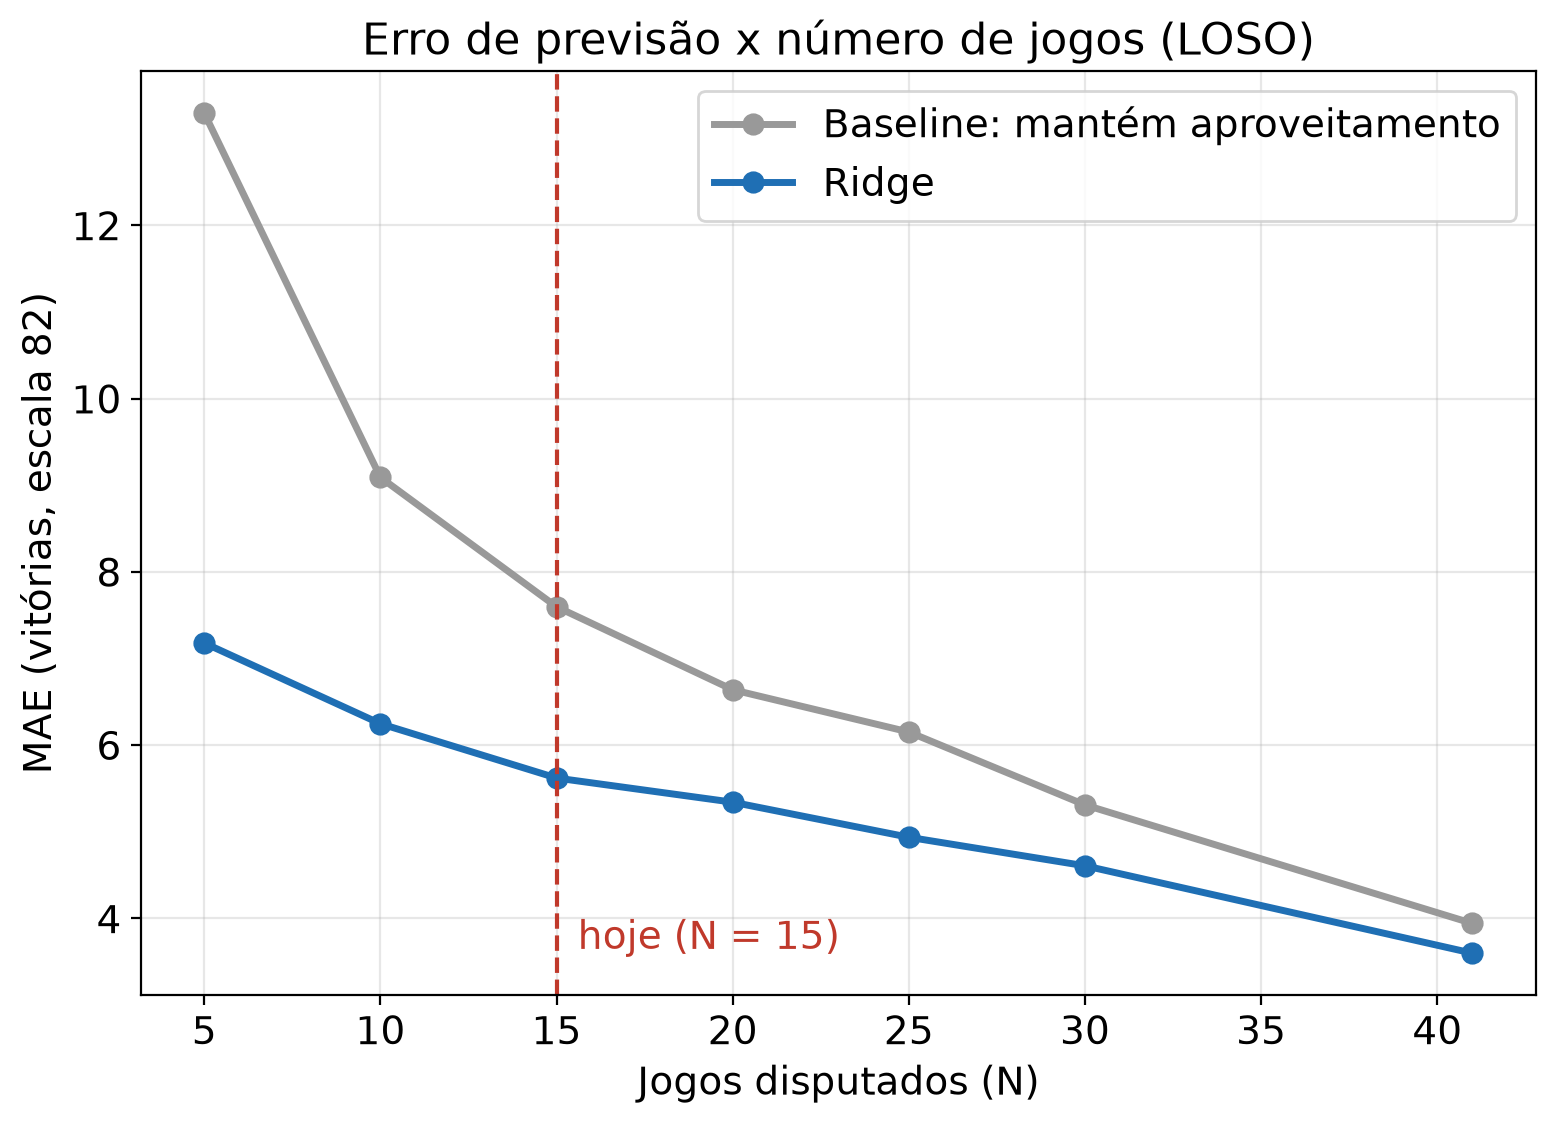
\includegraphics[width=0.9\columnwidth]{sensibilidade_n.png}}
\caption{MAE leave-one-season-out em função do número de jogos usados para construir as features.}
\label{fig:sens}
\end{figure}

\subsection{Simulação}
O modelo de jogo ajustado tem $b_{\Delta}=4{,}35$ e $b_h=0{,}32$, isto é, probabilidade de 57,9\% de vitória do mandante entre times iguais; sua acurácia nos jogos de treino é de 64,3\% (log-loss 0,629). A Eq.~\eqref{eq:sigma} dá $\sigma=0{,}085$. No backtest fora da amostra, os intervalos de 80\% contêm o número real de vitórias em 81,0\% dos 480 times-temporada, e o Brier score de três classes é 0,421, contra 0,658 de probabilidades constantes (6/15, 4/15, 5/15). A Fig.~\ref{fig:calib} mostra que as frequências previstas e observadas acompanham a diagonal de perto.

\begin{figure}[t]
\centerline{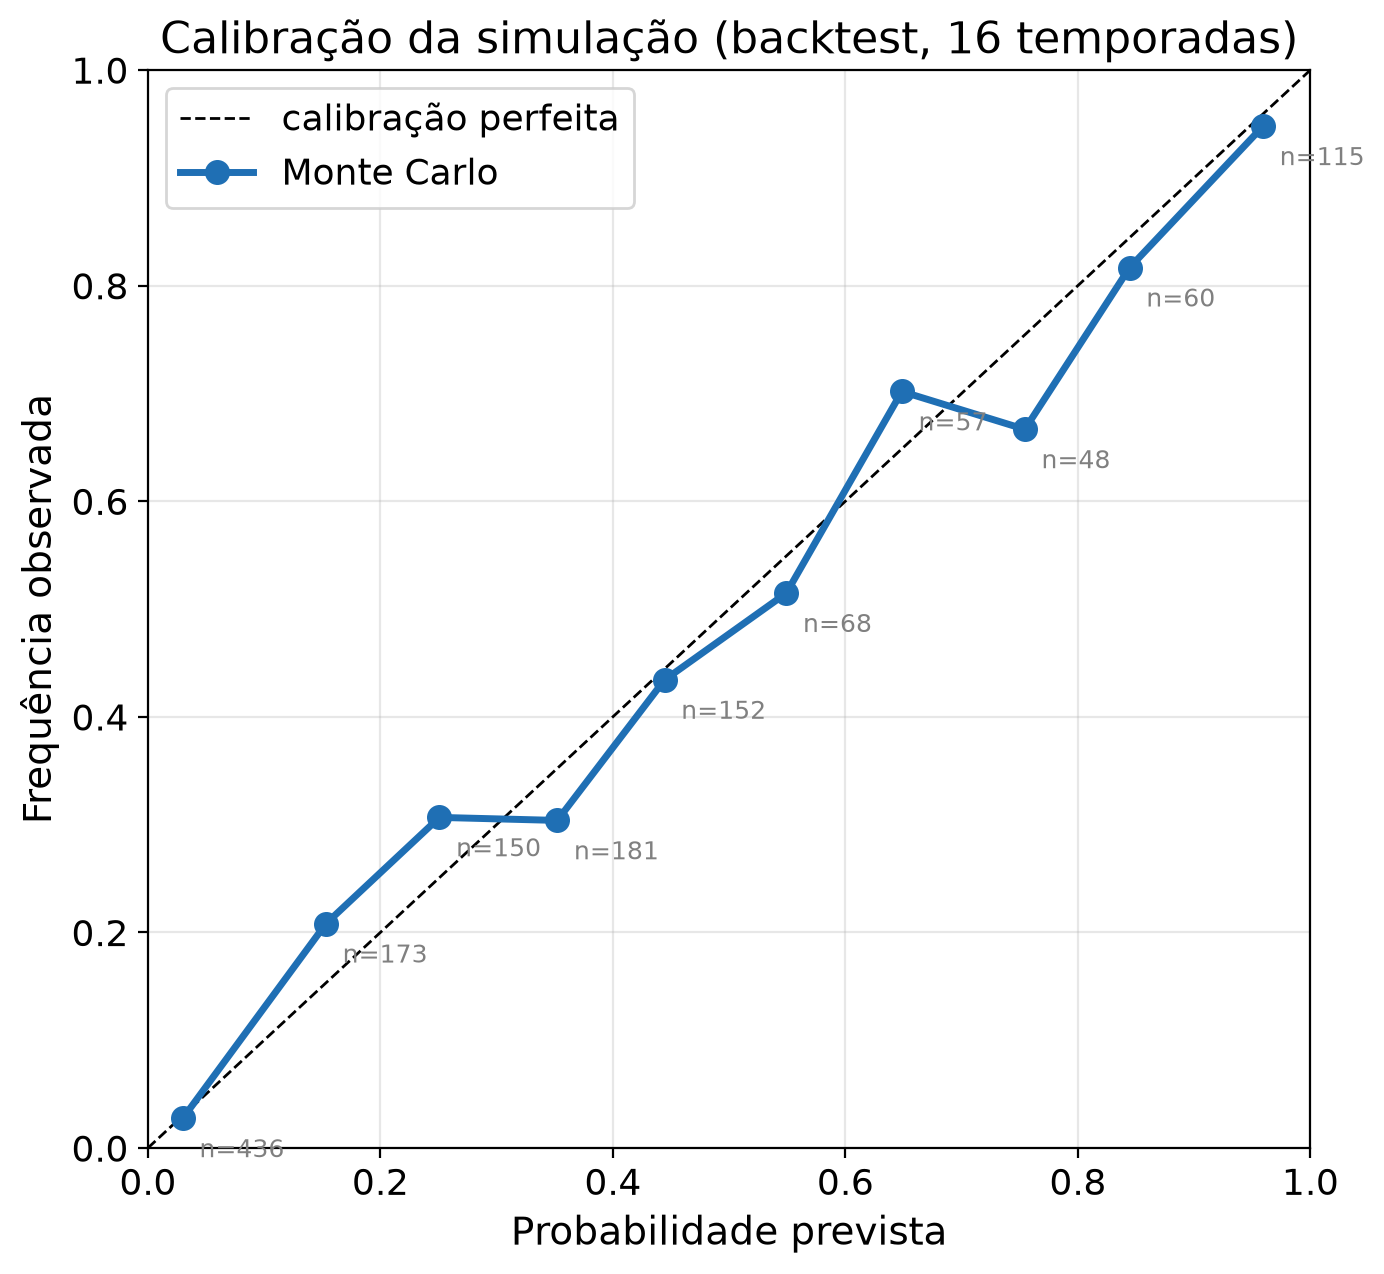
\includegraphics[width=0.8\columnwidth]{calibracao_simulacao.png}}
\caption{Calibração das probabilidades simuladas de top 6, play-in e fora no backtest fora da amostra (16 temporadas, faixas de largura 0,1; $n$ = número de pares time-classe).}
\label{fig:calib}
\end{figure}

\subsection{Projeção 2026--27}
A Tabela~\ref{tab:proj} e a Fig.~\ref{fig:heat} mostram a projeção em 22 de novembro de 2026. Boston (97\% de top 6) e San Antonio (95\%) são os favoritos mais claros. O modelo também modera começos fortes: o Philadelphia está 14--3, mas a projeção é de 52,4 vitórias, porque seu saldo de pontos é modesto; o Memphis, 12--5 após uma temporada de 25 vitórias, tem só 48\% de chance de terminar entre os seis primeiros. Na parte de baixo, Sacramento e Utah têm menos de 1\% de chance de chegar sequer ao play-in.

\begin{table*}[t]
\caption{Projeção 2026--27 (10.000 simulações, em 22/11/2026): campanha atual, vitórias esperadas, intervalo de 80\% e probabilidades (\%) de top 6, play-in e fora}
\begin{center}
\footnotesize
\setlength{\tabcolsep}{4.2pt}
\begin{tabular}{rlccccccrlcccccc}
\toprule
\multicolumn{8}{c}{\textbf{Conferência Leste}} & \multicolumn{8}{c}{\textbf{Conferência Oeste}} \\
\cmidrule(lr){1-8}\cmidrule(lr){9-16}
\# & Time & V--D & E[V] & Int. 80\% & Top 6 & Play-in & Fora & \# & Time & V--D & E[V] & Int. 80\% & Top 6 & Play-in & Fora \\
\midrule
1 & BOS & 11--6 & 55{,}8 & 48--63 & 97 & 3 & 0 & 1 & SAS & 14--3 & 58{,}9 & 51--66 & 95 & 5 & 0 \\
2 & DET & 10--6 & 53{,}6 & 46--61 & 94 & 6 & 0 & 2 & LAL & 14--3 & 55{,}8 & 48--63 & 86 & 14 & 0 \\
3 & PHI & 14--3 & 52{,}4 & 44--60 & 90 & 9 & 0 & 3 & HOU & 12--5 & 54{,}5 & 47--62 & 82 & 17 & 1 \\
4 & NYK & 11--6 & 50{,}9 & 43--59 & 86 & 13 & 0 & 4 & MIN & 12--5 & 54{,}3 & 46--62 & 81 & 18 & 1 \\
5 & ATL & 11--6 & 46{,}5 & 38--55 & 67 & 32 & 1 & 5 & OKC & 10--7 & 50{,}5 & 43--58 & 61 & 36 & 3 \\
6 & CLE & 9--8 & 45{,}7 & 37--54 & 62 & 36 & 2 & 6 & POR & 10--6 & 50{,}2 & 42--58 & 59 & 38 & 3 \\
7 & MIA & 10--6 & 45{,}6 & 37--54 & 61 & 37 & 2 & 7 & MEM & 12--5 & 48{,}5 & 40--57 & 48 & 46 & 6 \\
8 & TOR & 6--10 & 38{,}1 & 30--47 & 19 & 65 & 16 & 8 & DEN & 10--5 & 48{,}5 & 40--57 & 47 & 47 & 6 \\
9 & ORL & 7--9 & 38{,}0 & 29--47 & 18 & 65 & 16 & 9 & GSW & 9--8 & 43{,}2 & 35--51 & 19 & 60 & 21 \\
10 & IND & 5--12 & 30{,}7 & 23--39 & 3 & 41 & 56 & 10 & PHX & 8--7 & 41{,}8 & 33--50 & 14 & 57 & 29 \\
11 & CHI & 4--12 & 28{,}2 & 20--36 & 1 & 28 & 71 & 11 & DAL & 10--7 & 39{,}7 & 32--48 & 8 & 51 & 42 \\
12 & CHA & 4--11 & 27{,}8 & 20--36 & 1 & 26 & 73 & 12 & LAC & 4--11 & 29{,}5 & 21--38 & 0 & 8 & 92 \\
13 & WAS & 7--11 & 27{,}7 & 20--35 & 0 & 24 & 76 & 13 & NOP & 5--13 & 26{,}6 & 19--34 & 0 & 3 & 97 \\
14 & BKN & 3--12 & 24{,}0 & 17--32 & 0 & 11 & 89 & 14 & UTA & 3--15 & 23{,}2 & 16--31 & 0 & 1 & 99 \\
15 & MIL & 1--16 & 20{,}2 & 13--28 & 0 & 3 & 97 & 15 & SAC & 2--14 & 19{,}7 & 13--27 & 0 & 0 & 100 \\

\bottomrule
\end{tabular}
\label{tab:proj}
\end{center}
\end{table*}

\begin{figure*}[t]
\centerline{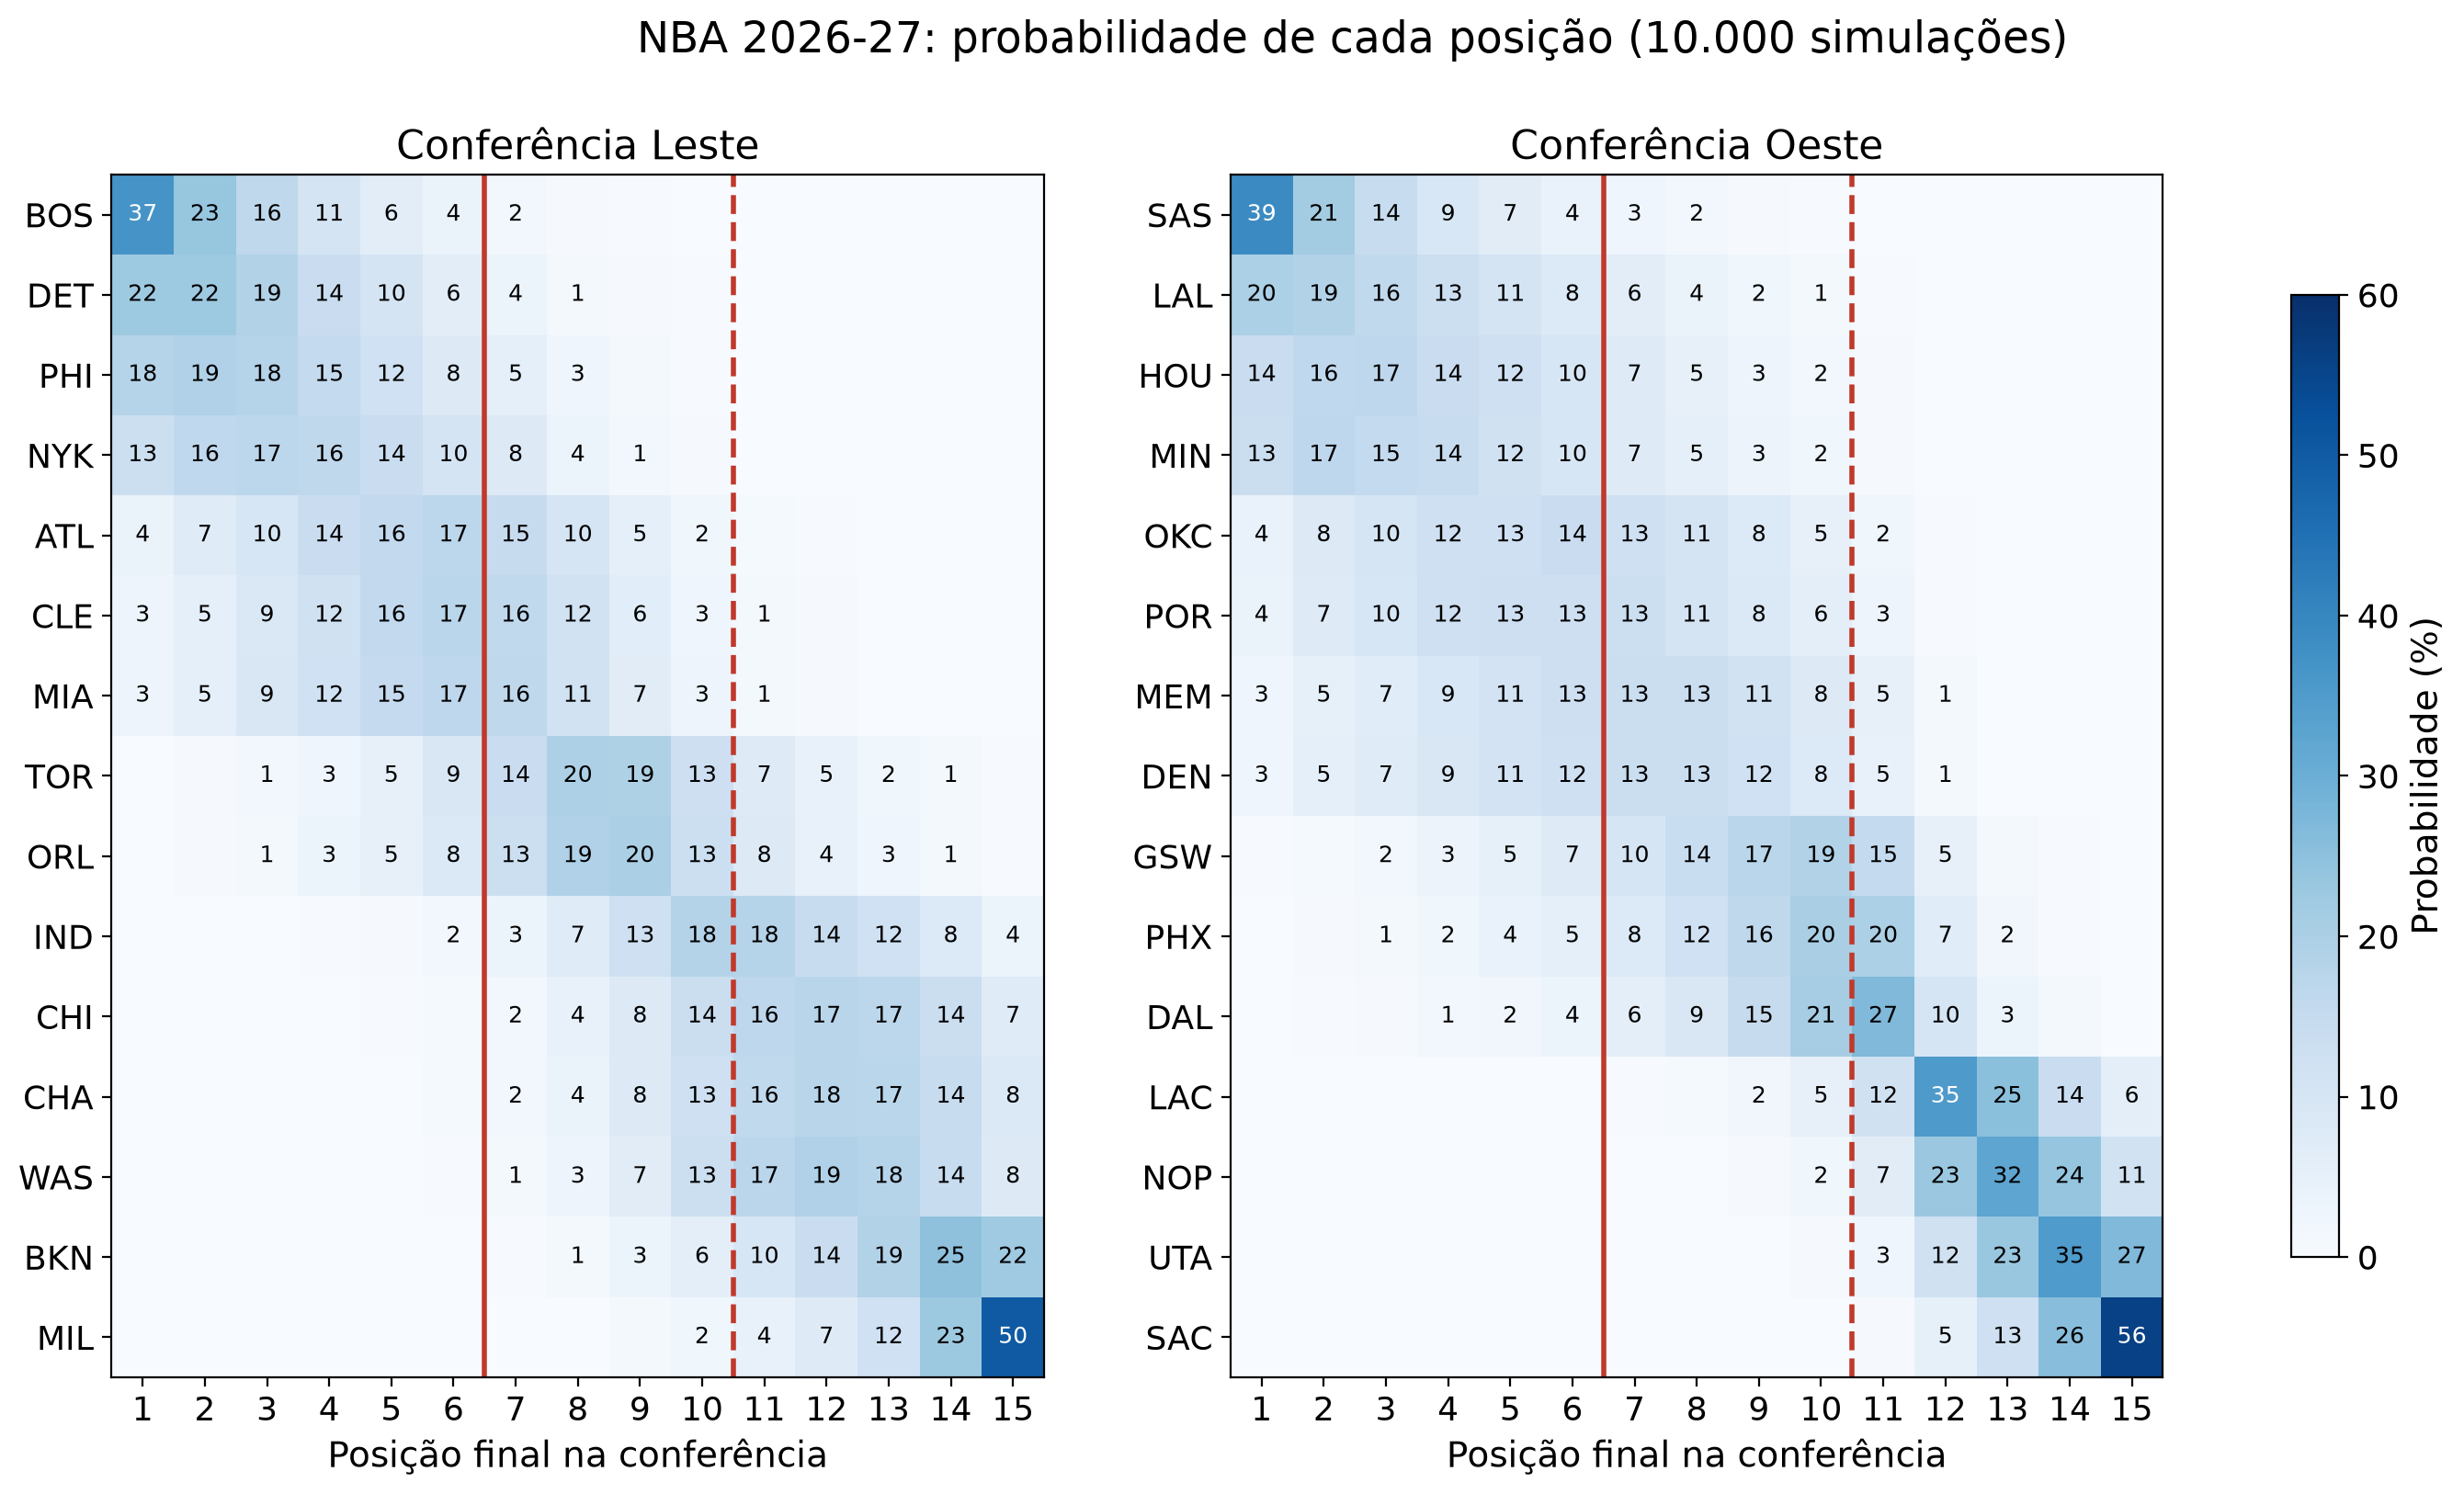
\includegraphics[width=0.92\textwidth]{heatmap_posicoes.png}}
\caption{Probabilidade (\%) de cada posição final na conferência em 2026--27. Linha contínua: corte do top 6; linha tracejada: corte do play-in.}
\label{fig:heat}
\end{figure*}

%=====================================================================
\section{Discussão}
O principal achado é que \emph{como} as campanhas iniciais são encolhidas importa mais do que \emph{qual} algoritmo é usado: quando o modelo pode puxar a campanha em direção à média e combiná-la com saldo de pontos e temporada anterior, OLS, Ridge, Lasso e random forest são estatisticamente indistinguíveis, e todos superam os baselines ingênuos com folga. A random forest não melhora os modelos lineares, o que é coerente com uma relação quase linear (Fig.~\ref{fig:rtm}) e com uma amostra pequena (480 linhas). O Ridge foi preferido não pela precisão, mas pela estabilidade: seus coeficientes são interpretáveis e robustos à colinearidade quase exata entre as features de pontos, que é a motivação clássica da regularização $\ell_2$. Note que a regressão à média em si é capturada por qualquer modelo linear, por meio de uma inclinação menor que um e de um intercepto em 0,500; a penalidade acrescenta estabilidade aos coeficientes, não um encolhimento adicional em direção a 0,500.

O baseline Pythagorean supera a campanha bruta, confirmando que o saldo de pontos é um sinal de força menos ruidoso do que vitórias e derrotas. A força de tabela após 15 jogos quase não traz informação, provavelmente porque as campanhas dos adversários também são ruidosas nesse ponto.

O backtest é a evidência mais forte de que as probabilidades são confiáveis: os intervalos têm a cobertura nominal e a curva de calibração acompanha a diagonal. Sem o termo de incerteza do rating, a simulação trataria as previsões como exatas e os intervalos ficariam estreitos demais.

\paragraph*{Limitações} (i) Com 15 jogos, mesmo o melhor modelo erra em média cerca de 5,6 vitórias; uma única lesão pode mudar mais do que isso. (ii) Lesões, trocas e mudanças de elenco não são modeladas; os ratings dependem só dos resultados. (iii) Os ratings são estáticos: usam apenas os 15 primeiros jogos, para casar com o treino, de modo que o 16º ao 18º jogos de quem já os disputou contam como vitórias, mas não atualizam o rating. (iv) Empates são desfeitos aleatoriamente, e não pelos critérios oficiais da NBA. (v) Os dois jogos da NBA Cup ainda não marcados são simulados contra um adversário médio, e jogos em quadra neutra são tratados como jogos com mando normal. (vi) A vantagem de jogar em casa é suposta constante entre temporadas, inclusive em 2020--21, disputada em grande parte sem público.

%=====================================================================
\section{Conclusão}
Quinze jogos não são uma temporada, mas também não são inúteis. Um modelo linear regularizado com seis features simples reduz em um quarto o erro da previsão ingênua ``campanha atual'' (de 7,6 para 5,6 vitórias), e quase pela metade após apenas cinco jogos. Combinado com um modelo logístico de jogo, incerteza no rating e simulação de Monte Carlo, ele produz probabilidades calibradas de top 6, play-in e eliminação para a temporada 2026--27. Extensões naturais são informações por jogador (lesões, minutos, trocas), ratings atualizados jogo a jogo e os critérios oficiais de desempate.

%=====================================================================
\section*{Contribuições dos Autores}
[A ser preenchido pelos autores. Exemplo: A1 definiu a pergunta de pesquisa e o plano do projeto, coletou os dados e escreveu o artigo; A2 implementou os modelos e a simulação, produziu as figuras e preparou a apresentação. Todos os autores revisaram a versão final.]

\section*{Declaração de Uso de IA}
O Claude (Anthropic), por meio da ferramenta Claude Code, foi usado neste projeto para implementar e depurar o código Python (coleta de dados, features, modelos, simulação e figuras) seguindo um plano em fases escrito pelos autores; para revisar a metodologia, o que levou à regra de um erro-padrão para $\alpha$ e ao backtest fora da amostra da simulação; e para redigir este artigo e os slides da apresentação em inglês e português. Os autores definiram a pergunta de pesquisa, a fonte de dados, as features, os modelos e o protocolo de validação, conferiram os resultados executando o notebook e são responsáveis por todo o conteúdo. [Autores: ajustem esta declaração ao uso real.]

\begin{thebibliography}{00}
\bibitem{efron1975} B. Efron and C. Morris, ``Data analysis using Stein's estimator and its generalizations,'' \textit{J. Amer. Statist. Assoc.}, vol. 70, no. 350, pp. 311--319, 1975.
\bibitem{efron1977} B. Efron and C. Morris, ``Stein's paradox in statistics,'' \textit{Scientific American}, vol. 236, no. 5, pp. 119--127, 1977.
\bibitem{hoerl1970} A. E. Hoerl and R. W. Kennard, ``Ridge regression: biased estimation for nonorthogonal problems,'' \textit{Technometrics}, vol. 12, no. 1, pp. 55--67, 1970.
\bibitem{tibshirani1996} R. Tibshirani, ``Regression shrinkage and selection via the lasso,'' \textit{J. Roy. Statist. Soc. B}, vol. 58, no. 1, pp. 267--288, 1996.
\bibitem{breiman2001} L. Breiman, ``Random forests,'' \textit{Machine Learning}, vol. 45, no. 1, pp. 5--32, 2001.
\bibitem{metropolis1949} N. Metropolis and S. Ulam, ``The Monte Carlo method,'' \textit{J. Amer. Statist. Assoc.}, vol. 44, no. 247, pp. 335--341, 1949.
\bibitem{nbaapi} S. Patel \textit{et al.}, ``nba\_api: an API client package to access the APIs for NBA.com,'' 2024. [Online]. Disponível em: \url{https://github.com/swar/nba_api}
\bibitem{kubatko2007} J. Kubatko, D. Oliver, K. Pelton, and D. T. Rosenbaum, ``A starting point for analyzing basketball statistics,'' \textit{J. Quant. Anal. Sports}, vol. 3, no. 3, 2007.
\bibitem{islr2021} G. James, D. Witten, T. Hastie, and R. Tibshirani, \textit{An Introduction to Statistical Learning}, 2nd ed. New York: Springer, 2021.
\bibitem{esl2009} T. Hastie, R. Tibshirani, and J. Friedman, \textit{The Elements of Statistical Learning}, 2nd ed. New York: Springer, 2009.
\bibitem{sklearn} F. Pedregosa \textit{et al.}, ``Scikit-learn: machine learning in Python,'' \textit{J. Mach. Learn. Res.}, vol. 12, pp. 2825--2830, 2011.
\bibitem{bradley1952} R. A. Bradley and M. E. Terry, ``Rank analysis of incomplete block designs: I. The method of paired comparisons,'' \textit{Biometrika}, vol. 39, no. 3/4, pp. 324--345, 1952.
\bibitem{brier1950} G. W. Brier, ``Verification of forecasts expressed in terms of probability,'' \textit{Monthly Weather Review}, vol. 78, no. 1, pp. 1--3, 1950.
\end{thebibliography}

\end{document}
